\documentclass[11pt]{article}
\usepackage[margin=1in]{geometry}
\usepackage{amsmath,amssymb,amsthm,booktabs,enumitem,xcolor,graphicx}
\setlist[itemize]{label=$\bullet$}
\usepackage[hidelinks]{hyperref}
\newtheorem{theorem}{Theorem}\newtheorem{proposition}[theorem]{Proposition}\newtheorem{lemma}[theorem]{Lemma}
\theoremstyle{definition}\newtheorem{hypothesis}{Hypothesis}\newtheorem{prediction}{Prediction}
\theoremstyle{remark}\newtheorem{remark}[theorem]{Remark}
\newcommand{\grade}[1]{\textsf{\small[#1]}}
\setlength{\parskip}{0.3em}
\title{The Neutrinos at the Wall:\\ Mass, Decoupling, and a Record That Passes Through the Fold}
\author{Jeromie Beasley}
\date{14 November 2026}
\begin{document}
\maketitle

\noindent\emph{AI-assisted. The ideas and research direction are the author's. AI tools (Claude, Anthropic) were used for literature search, computation, drafting and typesetting. Every number not taken from the author's archived runs is computed by the scripts \texttt{wall\_checks.py} and \texttt{fig\_wall.py}, described in Appendix~C. Grades: \grade{derived} proved here or in the cited paper of the author; \grade{measured} computed from runs; \grade{reading} an interpretation; \grade{H} a hypothesis with a stated test.}

\begin{abstract}
One wall organises this paper. In the author's link coordinate $\Gamma=\tanh(\tfrac12\ln z)$, two equal perpendicular steps of ratio $z$ have a commutator of trace $2-4\sinh^4(\tfrac12\ln z)$. That commutator turns parabolic, the boundary between turning and passing, at exactly $z=3+2\sqrt2$, $\Gamma^2=\tfrac12$.

The neutrinos sit on this wall twice. First, in their masses. With the lightest neutrino massless, the current oscillation data give $m_3/m_2=5.807\pm0.052$, which is $0.41\sigma$ from $3+2\sqrt2=5.8284$ (NuFIT~6.0 alone: $5.8165\pm0.079$, $0.15\sigma$). On the wall's own picture, the square of two such steps is a turn whose centre sits near the rim, while every charged step's square is a run to the rim. Every charged-fermion generation step lies past the wall, $\Gamma$ from $0.89$ to $0.997$. Taking the neutrino step to lie on the wall exactly fixes:
\begin{itemize}[nosep]
\item normal ordering;
\item $m_2=8.65$ and $m_3=50.44$\,meV;
\item $\Sigma m_\nu=59.1$\,meV;
\item $\Delta m^2_{31}/\Delta m^2_{21}=(1+\sqrt2)^4=33.97$, against $33.72$ measured ($33.83$ on NuFIT~6.0);
\item a lightest mass below about $1.5$\,meV;
\item $m_\beta=8.85$\,meV and $m_{\beta\beta}\in[1.5,3.7]$\,meV.
\end{itemize}

Second, in how the neutrinos let go of the plasma. The isotropic sector of their transport operator has a kept mode only while the collision rate exceeds $\kappa=2k/\pi$. There its non-orthogonality $4\phi^2/\sin^22\phi$ diverges and the mode merges into free streaming. All the non-normality sits on the density--flux link, with weight equal to the sound speed. The neutrinos are the first species to cross this wall, at about $1$\,MeV, across an electron--positron layer that later heats only the light.

The record they carry across it is physical. In S.~McCormick's general-relativistic collapse code, two neutrino states identical in density, flux, stress and every metric quantity, differing only in hidden angular structure planted at decoupling, have black-hole thresholds up to $5.5\times10^{-3}$ apart. In a Gaussian universe, at the planted amplitude, that changes the number of black holes near $6\times10^5\,M_\odot$ by 5--47\%, with a sign set by the record's orientation; a record of random orientation still raises it, by up to 8\%. The planted amplitude is engineered, half of each cell's positivity margin, and only that amplitude was run.

Finally, the author's fold theorem, proved for four-body shape space and the static base of a horizon, applies to the radiation era itself. Cosmic time is the even observable and the conformal scale factor the signed one, so the apparent beginning is a fold at finite distance. The path continues through it to the mirror. The author's survival principles state what crosses: the contour ledger and the orientation. A universe that recurs through such folds can deliver the neutrinos to decoupling already carrying a record. A blank start cannot.

The paper states each prediction with the experiment that can refute it. It credits the prior work it meets: Alikhanov for the mass relation, Boyle, Finn and Turok for the mirror continuation and a massless lightest neutrino, and McCormick for the collapse code and the free-streaming effect.
\end{abstract}

\tableofcontents

\section{The claim}\label{sec:claim}

A wall, in the author's work, is not where something is stored. It is where a memory exerts force: what arrives across it is written in, and nothing written inside can write back~\cite{BH}. The author has met such walls in four-body shape space, in the static base of a horizon, at the innermost stable orbit of a black hole, in the Sun's dynamo, and at an optical threshold~\cite{BH,Light,Suns}. At each of them two things survive exactly, whatever happens to the individual eigenvectors: the contour's ledger and the orientation. \emph{The contour keeps the ledger; the orientation keeps the trace}~\cite{BH}.

This paper's claim is that the neutrinos are the particles at such a wall, in three ways that can be checked:
\begin{enumerate}[nosep]
\item their heaviest mass step lies on the wall $\Gamma^2=\tfrac12$ where a pair of equal perpendicular steps turns parabolic (Section~\ref{sec:masses});
\item their decoupling is the same kind of wall in motion. The kept sector of their transport loses its mode at $\kappa=2k/\pi$, and they are the first species to cross (Section~\ref{sec:letgo});
\item the record they carry across changes how many black holes form (Section~\ref{sec:bh}), and a universe that passes through a fold rather than beginning can supply that record (Section~\ref{sec:fold}).
\end{enumerate}
Section~\ref{sec:tests} collects every prediction with the measurement that can refute it. Section~\ref{sec:notclaimed} says what is not claimed.

\section{The wall}\label{sec:wall}

\subsection{The link coordinate}
Two books, two rates, two masses: any positive pair $d_i,d_j$ forms a link with ratio $z=d_i/d_j$, rapidity $\tfrac12\ln z$ and Smith coordinate
\begin{equation}
\Gamma=\frac{z-1}{z+1}=\tanh\big(\tfrac12\ln z\big),\qquad \frac{E^-}{E^+}=\Gamma^2 ,
\end{equation}
where $E^\mp$ are the two books of the link~\cite{VOTKP,Atlas}. Exchanging the ends negates $\Gamma$. A matched link, $z=1$, sits at the centre of the chart. The same coordinate is the reflection coefficient of a wave at a change of spectral gap, $\Gamma=\tanh(\tfrac12\ln\Delta_2/\Delta_1)$~\cite{BH}, and the neutrino transport's flux--shear link $\Gamma_{12}=(r-1)/(r+1)$~\cite{NU10}.

\subsection{Where a pair of steps turns parabolic}
\begin{theorem}[the wall of two equal perpendicular steps]\label{thm:wall}\grade{derived; Appendix A.1; checked}
Let $B_x(r)$ and $B_y(r)$ be boosts of rapidity $r$ along perpendicular axes in $SL(2,\mathbb C)$, and $K=B_xB_yB_x^{-1}B_y^{-1}$ their commutator. Then
\begin{equation}
\operatorname{tr}K=2-4\sinh^4(r/2).
\end{equation}
$K$ is elliptic (a pure turn) for $\operatorname{tr}K\in(-2,2)$, parabolic at $\operatorname{tr}K=-2$, and loxodromic beyond. The parabolic wall is at
\begin{equation}
r_w=\ln(3+2\sqrt2)=1.762747,\qquad z_w=e^{r_w}=3+2\sqrt2=5.828427,\qquad \Gamma_w=\tanh(r_w/2)=\frac1{\sqrt2}.
\end{equation}
\end{theorem}
This is the author's BallJoins J3--J4, machine-checked in Lean (\texttt{line\_ratio}, \texttt{five\_inside\_seven\_outside}), and atlas cards B189 and B199~\cite{TwoTrees,Atlas,SMball}. Below $z_w$ a loop of two perpendicular steps closes as a turn: a bound orbit, a spin. Above it the loop climbs and turns: a flyby. On the wall it does neither: a Jordan block, the parabolic case. A black hole carries exactly this kind of wall at its innermost stable circular orbit, where the wobble generator of circular orbits squares to zero and gravity's effective power reaches the inverse cube, $p=2+6M/r=3$~\cite{BH}.

\paragraph{The wall seen from the balls.} The same wall has a picture in the author's ball~\cite{TwoTrees,Mixer}. Put a ball at the centre and a neighbour one step of ratio $z$ out along each of two perpendicular arms. Between the centre and each neighbour stands the face halfway, at rapidity $\tfrac12\ln z$. For two equal steps
\begin{equation}
g=\sinh^2\big(\tfrac12\ln z\big)=\frac{(z-1)^2}{4z}.
\end{equation}
\begin{proposition}[turn or run~\cite{TwoTrees}, Theorems 5.3, 5.4 and 8.4]\label{prop:turnrun}\grade{derived there; Lean BallJoins J3, J4, J7; checked, Appendix C}
If $g<1$ the two faces cross, at the angle $\arccos g$, and the square of the two steps (step $a$, step $b$, back $a$, back $b$) is a turn by $4\arccos g$ about a fixed point at
\begin{equation}
\tanh^2\frac{\rho}{2}=\frac{1-s}{1+s},\qquad s=\sqrt{1-2\Gamma^2}.
\end{equation}
Repeating it carries the centre round a ring: the walk is held. If $g>1$ the faces stand apart by $\operatorname{arccosh}g$ and the square is a run of length $4\operatorname{arccosh}g$: repeating it carries the centre to the rim. At $g=1$ the faces just touch, $s=0$, and the fixed point reaches the rim. This is the wall of Theorem~\ref{thm:wall}: $g=1$ is $\sinh(r/2)=1$. Reversing one step, or the order, reverses the sense of the turn.
\end{proposition}
The turn angle follows from Theorem~\ref{thm:wall}: the half-trace of the square is $1-2g^2=\cos(\pi-2\arccos g)$, so the turn is $2\pi-4\arccos g$, a turn of size $4\arccos g$ in the opposite sense.

\subsection{Two kinds of wall, and what survives}
The author sorts walls into two kinds~\cite{BH}.
\begin{itemize}[nosep]
\item At a \emph{spectral} wall a real pair of eigenvalues turns complex along a physical path, and the Jordan block is present in every frame. Examples: the innermost stable orbit, the Sun's dynamo wave, the optical threshold.
\item At a \emph{geometric} wall, or fold, the spectrum stays real on both sides. The block belongs only to the folded chart, and the path passes through to a mirror configuration. Examples: the coplanar wall of four-body shape space, the static base of a horizon.
\end{itemize}

\begin{theorem}[the fold~\cite{BH}, Theorem 2]\label{thm:fold}\grade{derived there}
Let an even observable $X$ be the square of a signed coordinate $\lambda$, $X=\lambda^2$. A metric that is regular and even in $\lambda$ reads $ds^2=dX^2/(4c^2X)$ in $X$. Its coefficient diverges at $X=0$, while the distance to the wall is finite and the path continues to $\lambda<0$, the mirror. On four-body shape space $c=1$ and the distance from the wall to $w_3=\varepsilon$ is $\arcsin\sqrt\varepsilon$. On the Schwarzschild static base $c=\kappa$, the surface gravity.
\end{theorem}

What passes a wall of either kind is fixed by two survival principles. Both are proved in~\cite{BH}.
\begin{itemize}[nosep]
\item The Riesz projector of the colliding pair and its trace-log ledger, $\log\det(c+A_{\rm pair})$, stay exact through the wall in every frame, where single eigenprojectors diverge like $|A_{12}|/\mathrm{gap}$.
\item The orientation, the sign of $\det X$ and the analytic label of the branch, survives as a $\mathbb Z_2$ record that the even observer cannot see. Readings odd under the mirror cancel across it; even readings survive.
\end{itemize}
Compression at a wall, $X\mapsto PXP$, is ``rank compression, not destruction''~\cite{BH}.

\section{The masses at the wall}\label{sec:masses}

\subsection{Charged fermions step past the wall}
Read as links, the generation steps of the charged fermions are all loxodromic. They lie past $z_w$, with $\Gamma$ from $0.888$ ($\mu\to\tau$, $z=16.8$) to $0.997$ ($u\to c$, $z=589$) \grade{measured, \cite{SMball}}. The charged leptons have a second structure. Koide's $Q=(m_e+m_\mu+m_\tau)/(\sqrt{m_e}+\sqrt{m_\mu}+\sqrt{m_\tau})^2$ is $0.6666644634$, so the vector $(\sqrt{m_e},\sqrt{m_\mu},\sqrt{m_\tau})$ makes an angle with $\cos^2=1/(3Q)=0.50000165$ with $(1,1,1)$~\cite{Koide}. In the author's atlas this is a link with \emph{balanced books}, $E^-=E^+$ (card B200)~\cite{Atlas}. It is a different condition from the wall $E^-/E^+=\tfrac12$ of card B189, and the two are not identified here \grade{reading}.

\subsection{The neutrinos' heaviest step is on the wall}
With normal ordering and $m_1=0$, the oscillation splittings fix $m_2=\sqrt{\Delta m^2_{21}}$ and $m_3=\sqrt{\Delta m^2_{31}}$. The NuFIT~6.0 central values~\cite{NuFIT} give
\begin{equation}
\frac{m_3}{m_2}=5.8165\pm0.079\quad\text{against}\quad z_w=3+2\sqrt2=5.8284,
\end{equation}
a difference of $-0.15\sigma$ \grade{measured, \cite{SMball}; recomputed, Appendix C}. Equivalently $\Delta m^2_{31}/\Delta m^2_{21}=33.83$ against $(1+\sqrt2)^4=33.97$. With the first JUNO measurement $\Delta m^2_{21}=(7.50\pm0.12)\times10^{-5}$\,eV$^2$ and NuFIT~6.1's $\Delta m^2_{31}=(2.529\pm0.021)\times10^{-3}$\,eV$^2$, the inputs Alikhanov uses~\cite{Alik}, the ratio is $33.72$ and
\begin{equation}
\frac{m_3}{m_2}=5.807\pm0.052,
\end{equation}
$-0.41\sigma$ from the wall \grade{computed, Appendix C}. The relation $(m_3+m_2)/(m_3-m_2)=\sqrt2$ with $m_1=0$ was proposed by Alikhanov~\cite{Alik}. It is the same number. What this paper adds is its place: it is the link $\Gamma^2=\tfrac12$ of Theorem~\ref{thm:wall}.

\begin{figure}[t]\centering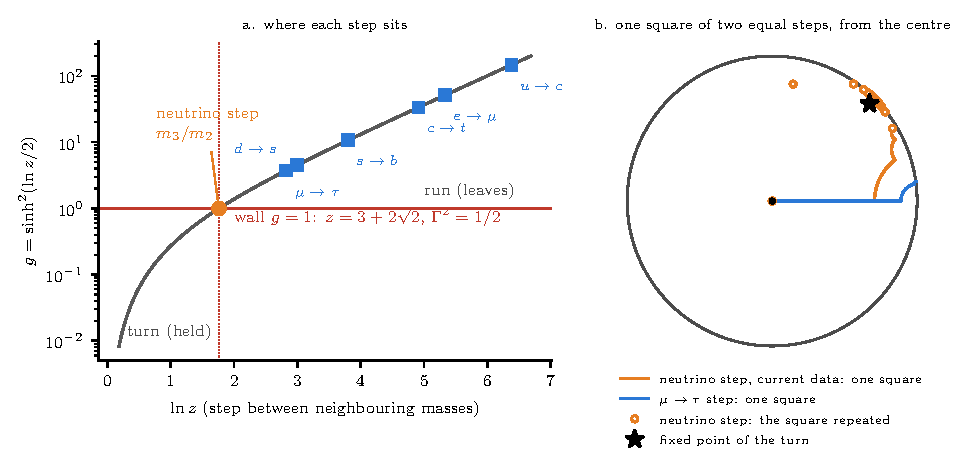
\includegraphics[width=\textwidth]{fig_wall.pdf}
\caption{The neutrino step at the wall. (a) $g=\sinh^2(\tfrac12\ln z)$ for each step between neighbouring masses. The wall $g=1$ is $z=3+2\sqrt2$; the neutrino step $m_3/m_2$ (both data sets) sits on it, every charged generation step lies past it. (b) One square of two equal steps from the centre of the ball, computed from the boost matrices. The neutrino step (current data) closes into a turn of $23.4^\circ$ about a fixed point near the rim (star, $\tanh(\rho/2)=0.950$); the square repeated walks the ring round it (open circles). The $\mu\to\tau$ step is a run of length $7.95$ that ends at the rim. Script \texttt{fig\_wall.py}.}\label{fig:wall}\end{figure}

The charged steps pass the wall. The neutrino step sits on it. Figure~\ref{fig:wall} shows both by Proposition~\ref{prop:turnrun}. With the measured step the square of two neutrino steps is a turn of $23.4^\circ$ (current data; $17.4^\circ$ on NuFIT~6.0) about a fixed point at $\tanh(\rho/2)=0.950$ ($0.963$): held, at the edge. The $\mu\to\tau$ step, the smallest charged step, gives a run of length $7.95$ \grade{computed, Appendix C}. Read in the ball, the neutrinos are held just inside the line, and every charged step runs out \grade{reading}. The neutrinos are also the particles that sit just inside the rim of the author's ball, the velocity space of one massive particle: at a common energy of 1\,MeV a $0.05$\,eV neutrino is $1-5\times10^{-8}$ from the rim~\cite{SMball}.

\begin{hypothesis}[the neutrino step is the wall]\label{hyp:mass}
The neutrino mass step is exactly parabolic, $m_3/m_2=3+2\sqrt2$, with $m_1$ negligible.
\end{hypothesis}

Why the neutrinos land on the wall rather than past it is not derived here. The reading the author's work offers is this. A wall is where a memory exerts force and does not store it. The neutrinos are the species whose whole role in the universe's history is to let go first and carry the record outward (Section~\ref{sec:letgo}). A step on the wall is the step that neither binds (turns) nor escapes (climbs) \grade{reading}.

\subsection{What the hypothesis fixes}
\begin{center}\begin{tabular}{lll}\toprule
quantity & value on the wall & status today\\\midrule
mass ordering & normal & favoured, not settled\\
lightest mass $m_1$ & $\lesssim1.5$\,meV (exact wall: $0$) & open\\
$m_2,\ m_3$ & $8.65$, $50.44$\,meV & consistent\\
$\Delta m^2_{31}/\Delta m^2_{21}$ & $(1+\sqrt2)^4=33.971$ & $33.72$ ($33.83$ NuFIT~6.0)\\
$\Delta m^2_{31}$ given $\Delta m^2_{21}$ & $2.544\times10^{-3}$\,eV$^2$ & $2.534\times10^{-3}$\\
$\Sigma m_\nu$ & $59.1$\,meV & below current cosmological bounds\\
$m_\beta$ & $8.85$\,meV & below KATRIN's reach\\
$m_{\beta\beta}$ (if Majorana) & $1.5$--$3.7$\,meV & floor for future searches\\\bottomrule\end{tabular}\end{center}
\grade{derived from Hypothesis~\ref{hyp:mass} with NuFIT 6.0 central values; Appendix C}.

The sensitivity to $m_1$ is steep. The measured step $\sqrt{(m_1^2+\Delta m^2_{31})/(m_1^2+\Delta m^2_{21})}$ falls to $5.779$ at $m_1=1$\,meV, $5.672$ at $2$\,meV and $5.061$ at $5$\,meV. On NuFIT~6.0 the wall therefore requires $m_1$ below about $2$\,meV. On the current inputs the pull reaches $-2\sigma$ at $m_1=1.5$\,meV, so the wall requires $m_1$ below about $1.5$\,meV. Inverted ordering gives a step near $1$, deep inside the wall.

Boyle, Finn and Turok predicted a massless lightest neutrino from an entirely different argument, CPT symmetry of the universe across the bang~\cite{BFT,BFT2}. Section~\ref{sec:fold} meets their construction again. Here it suffices that two independent routes ask for $m_1=0$, and the present one additionally fixes the ratio of the other two.

\section{Letting go: decoupling is the same wall in motion}\label{sec:letgo}

\subsection{The cut}
For one Fourier mode $k$ the linearised neutrino intensity evolves under $L=-ik\mu-\kappa(I-P)$. Here $P$ projects onto the isotropic part, the kept sector, and $\kappa$ is the collision rate~\cite{McC,NU10}. In the Legendre basis streaming links only neighbours, with weights $c_\ell=(\ell+1)/\sqrt{(2\ell+1)(2\ell+3)}$. Collisions are diagonal.
\begin{proposition}[the cut~\cite{NU10,CE}]\grade{derived there; Lean}
$\tfrac18\lVert[L,L^*]\rVert_F^2=\sum_\ell k^2c_\ell^2(D_{\ell+1}-D_\ell)^2$. For one rate all of it sits on the density--flux link, $\kappa^2k^2/3$. The weight across the cut is $\sqrt{E_B}=\lVert PH(I-P)\rVert=k/\sqrt3$, the radiation sound speed times $k$.
\end{proposition}
The kept sector therefore moves at the sound speed, while what leaves it moves at the speed of light.

\subsection{The kept mode exists only above a wall}
The isotropic part has the exact propagator $\langle0|(s-L)^{-1}|0\rangle=g/(1-\kappa g)$, with $g=k^{-1}\arctan[k/(s+\kappa)]$~\cite{NU10}. A kept mode is a pole, $\kappa g=1$.
\begin{theorem}[the decoupling wall~\cite{NU10}; onset of Romatschke~\cite{Rom}]\label{thm:onset}\grade{derived there}
With $\phi=k/\kappa$ the kept mode is $s=k\cot\phi-\kappa$. It exists only for $\phi<\pi/2$, that is $\kappa>2k/\pi$. Its non-orthogonality, the squared ratio of its norm to its bilinear self-pairing, is
\begin{equation}
K=\frac{4\phi^2}{\sin^22\phi},
\end{equation}
equal to $1$ for a fully coupled gas and divergent at the wall, where the mode meets the branch cut of $g$ at its centre and merges into free streaming.
\end{theorem}
$K$ rises from $1.41$ at $\phi=0.5$ to $4.84$ at $\phi=1$, $69.9$ at $\phi=1.4$ and $5558$ at $\phi=1.55$ \grade{derived; Appendix C}. As the universe cools, $\kappa/k$ falls through $2/\pi$ for each scale in turn. That is the wall in motion. Before it the gas relaxes everything but the kept sector, and hidden structure is wiped. After it the gas lets go.

\subsection{The neutrinos are first, and an electron layer lies between}
The neutrinos cross this wall at a temperature of about $1$\,MeV. The photons cross their own, against the electrons, only near $0.26$\,eV. Between the two lies the electron--positron plasma. The neutrinos let go of it first. Then its annihilation near $0.5$\,MeV heats the photons and not the neutrinos~\cite{Dolgov}. The ordering is: neutrino side, electron layer, light side \grade{cited physics}. The author's own boundary work treats the laboratory version of such a layer, the electron screening cloud at a nuclear barrier~\cite{Screen}.

The neutrinos are fermions, and that fixes what their outside record can be. For a fermion pair the outside occupation $C$ has a definite offset
\begin{equation}
\tau=\log\frac{1-C}{C}=\frac{\hbar\omega}{k_BT},\qquad \Gamma=\tanh\frac{\hbar\omega}{2k_BT},
\end{equation}
for every pair phase, a point on the same Smith chart as the wall~\cite{BH,Offset}. A boson record has no ``full'' state and no such offset. Light and the neutrinos are the boson and fermion sides of one thermal record \grade{derived in~\cite{BH}; reading}. At decoupling the typical neutrino ($\hbar\omega\approx3.15\,k_BT$) sits at $\Gamma=0.918$, far out on the chart \grade{derived}.

\subsection{Where the record lives}
A fluid closure keeps density, flux and stress ($\ell\le2$). The author proved that eliminating the hidden moments $\ell\ge1$ exactly gives the kept amplitude one equation,
\begin{equation}
\dot a(t)=S(t)-k^2\!\int_s^tK(t,r)\,a(r)\,dr,
\end{equation}
with the whole hidden past in one source $S$ and one memory kernel $K$~\cite{NU10}. The kept population obeys the speed limit $\dot A^2\le4E_BA(1-A)$~\cite{NU10} \grade{derived there; Lean}. Hidden structure planted while the gas is coupled is erased by $\exp[-\epsilon_{\rm dec}^n/(n\tau_s^n)]$. Planted at or after decoupling, it returns into density, flux and stress at the several-per-cent level. The readout Gramian of the hidden sector has no kernel, so every hidden direction is eventually seen. Its spectrum ranks them: $10^{-7}$ in the coupled era, $0.37$ at decoupling, led by $\ell=3$~\cite{NU10} \grade{measured there}.

\section{What the record does to black holes}\label{sec:bh}

\subsection{The threshold reads the hidden record}
McCormick showed that free-streaming neutrinos raise the threshold for primordial black-hole formation, by about $0.235R_\nu$ in the linear compaction, and that the effect fades as decoupling becomes gradual~\cite{McC}. The author ran McCormick's public general-relativistic code to the decoupling surface and changed only the hidden part of the angular intensity~\cite{NU10}. The two matched states agree in their $\ell\le2$ moments to $4\times10^{-16}$, in the lapse and constraints to $10^{-15}$, and bit for bit in every fluid and metric array. Their thresholds:
\begin{center}\begin{tabular}{llcc}\toprule
planted at & hidden direction & $\delta_c(+)-\delta_c(-)$ & shift from unperturbed\\\midrule
coupled era & $\ell=3$, $\ell=4$ & $1.8\times10^{-5}$ & ---\\
decoupling & $\ell=3$ & $+3.74\times10^{-3}$ & $+1.83$ / $-1.91\times10^{-3}$\\
decoupling & $\ell=4$ & $-2.10\times10^{-3}$ & $-1.08$ / $+1.02\times10^{-3}$\\
decoupling & Gramian's leading direction & $+5.51\times10^{-3}$ & $+2.69$ / $-2.82\times10^{-3}$\\\bottomrule\end{tabular}\end{center}
The decoupling differences are 200 bracket widths or more and survive the resolution allowance \grade{measured, \cite{NU10}}. The threshold reads angular information that no closure on density, flux and stress holds. The response is close to odd in the amplitude. Odd structure moves the threshold $1.8$ times more than even, and the Gramian's ranking carries into the nonlinear collapse at about $60\%$ of its linear size.

\emph{Why the sign matters} \grade{reading}. Streaming climbs the chain one rung at a time. Odd hidden structure returns first as flux, a net neutrino push out of the overdensity or into it. Even structure returns first as stress, a radial pressure above or below the tangential. Outward push and radial pressure resist collapse; their opposites ease it.

\subsection{How many black holes}
For Gaussian fluctuations $\beta=\mathrm{erfc}[\delta_c/(\sqrt2\sigma)]$. Tune $\sigma$ so the unperturbed $\delta_c=0.51075$ gives $\beta_0$:
\begin{center}\begin{tabular}{lccc}\toprule
hidden record at decoupling & $\beta/\beta_0$ ($10^{-6}$) & ($10^{-10}$) & ($10^{-16}$)\\\midrule
$\ell=3$, either orientation & $0.91$ / $1.10$ & $0.86$ / $1.17$ & $0.78$ / $1.30$\\
$\ell=4$, either orientation & $1.05$ / $0.95$ & $1.09$ / $0.92$ & $1.16$ / $0.87$\\
Gramian direction, either orientation & $0.88$ / $1.15$ & $0.80$ / $1.27$ & $0.69$ / $1.47$\\
Gramian direction, random orientation & $1.012$ & $1.032$ & $1.081$\\\midrule
flux--shear split, McCormick's model & $0.99$ & $0.97$ & $0.96$\\\bottomrule\end{tabular}\end{center}
\grade{estimate: standard Gaussian abundance on the measured shifts; Appendix C}. A record invisible to every fluid and metric quantity at decoupling changes the number of black holes by 5--47\% at the planted amplitude. That is about three to eleven times what the flux--shear split does in McCormick's physical collision model~\cite{NU10}. Because $\beta$ is convex in $\delta_c$, a record of random orientation does not average away: it raises the abundance, by 0.3--1.4\% for $\ell=4$, 0.6--3.8\% for $\ell=3$ and 1.2--8.1\% along the Gramian's leading direction, and rarer black holes gain more. Two cautions. McCormick sets abundance with the linear compaction rather than the compaction peak used here. And the amplitudes are half each cell's positivity margin, chosen for the test; only that amplitude was run, so how the shift, and every number in the table, scales with the size of the record is untested.

\subsection{Where in mass}
With $M_H(T)\simeq1.5\times10^5M_\odot(T/\mathrm{MeV})^{-2}$ ($g_*=10.75$) and $\epsilon\propto1/T$, a perturbation whose collisions switch off at $\epsilon_{\rm dec}$ has mass $M\simeq\epsilon_{\rm dec}^2M_H(T_{\rm dec})$. The decoupling runs ($\epsilon_{\rm dec}=2$, $T_{\rm dec}\approx1$\,MeV) sit near $6\times10^5M_\odot$, where McCormick's step in the mass function begins. Supermassive black-hole seeds sit in this range~\cite{Dave} \grade{estimate}.

\section{Through the fold}\label{sec:fold}

\subsection{The radiation era is a fold}
In a flat radiation-dominated universe the scale factor is linear in conformal time, $a(\eta)=a_1\eta$, and cosmic time is $t=\int a\,d\eta=a_1\eta^2/2$. Cosmic time is the even observable and $\eta$ the signed coordinate: $t=X$, $\eta\propto\lambda$, exactly the setting of Theorem~\ref{thm:fold}. Read in $t$, $a=\sqrt{2a_1t}$ and $da/dt=a_1/\sqrt{2a_1t}$ diverges at $t=0$, the coefficient blow-up of the fold. Read in $\eta$, $a$ is analytic and odd, and nothing breaks: the path continues to $\eta<0$ \grade{derived; Appendix A.2}. An observer who records only even quantities sees a beginning, as the Gram observer of the four-body wall sees a bounce. In the signed coordinate it is a fold at finite distance, and the far side is the mirror.

Boyle, Finn and Turok used this analytic continuation to propose that the universe before the bang is the CPT image of the one after it, a universe/anti-universe pair, with $a(\eta)$ odd~\cite{BFT,BFT2}. The author arrived at the same structure independently, as a theorem about folds in four-body shape space and the static base of a horizon~\cite{BH}. What the author's work adds is what crosses the fold. That is the subject of the rest of this section.

\subsection{What passes through}
The two survival principles of Section~\ref{sec:wall} apply to any fold. The contour ledger passes unchanged. The orientation passes as a $\mathbb Z_2$ sign that the even observer cannot read. Readings odd under the mirror cancel across it, while even readings survive~\cite{BH}. In the author's words, what passes is ``all that can get compressed and still remain allowed a new rewinding after'' \grade{the author's statement, 14 November 2026}.

\begin{hypothesis}[recurrence]\label{hyp:cycle}
The universe is a self-recurring transport system: closed but growing, relaxing toward full relaxation, then letting go again through a fold. At each passage the compression keeps the ledger and the orientation, and the next cycle starts with what was kept.
\end{hypothesis}
Full relaxation is the coupled era taken to its end: everything but the kept sector damped, the door shut. Letting go is the wall of Theorem~\ref{thm:onset}. The first to let go are the lightest massive carriers, the neutrinos. ``Light leaves the lightest trail; all else follows and carves'' \grade{the author's statement}.

\subsection{What the two starts predict}
A blank start, with hidden moments empty at decoupling, is the standard assumption, and McCormick's runs and the author's memory curves begin that way. A recurrent start delivers the neutrinos to decoupling already carrying a record. The door of Section~\ref{sec:bh} then writes it into the threshold.
\begin{prediction}[the neutrino step in the black-hole mass function]\label{pred:mf}
Blank start: the mass function across $10^5$--$10^7M_\odot$ follows McCormick's step with no further shift. Recurrent start: if the carried record is coherent in orientation over the scales that form black holes, the abundance across the step shifts by tens of per cent, up or down according to its parity. If it is incoherent, the step is raised by a few per cent and its edge broadened.
\end{prediction}
\begin{prediction}[the parity of what survives]\label{pred:parity}\grade{H}
If each passage is the mirror fold of Theorem~\ref{thm:fold}, odd parts of the carried record cancel across it and even parts survive. The carried neutrino record is then even-led ($\ell=4$-type rather than $\ell=3$-type). Its effect on the abundance is bounded by the even row of the table in Section~\ref{sec:bh}, $\pm5$--$16\%$ coherent and $+0.3$--$1.4\%$ random.
\end{prediction}
Prediction~\ref{pred:parity} is sharper than the general recurrence statement and is the first place it can fail. It identifies the fold's mirror parity ($\eta\to-\eta$) with the angular parity of the record ($\ell$ odd or even, $\mu\to-\mu$); that identification is not derived here and is untested. Whether the next cycle is the mirror of this one or the same way round is left to the data. The two options give different parity content.

\subsection{How this differs from earlier cycles}
Penrose's conformal cyclic cosmology joins aeons through conformal geometry, with the carrier being the conformal structure of the boundary~\cite{CCC}. Steinhardt and Turok's cyclic model joins them through colliding branes~\cite{ST}. Boyle, Finn and Turok's universe is a single CPT pair~\cite{BFT}. Here the carrier is a kept transport sector with a measured channel, the door, by which a hidden record reaches matter. The fold is a theorem of the author's operator geometry, not an input. What crosses it is fixed by the same survival principles that govern black-hole walls.

\section{Tests}\label{sec:tests}
\begin{center}\small\begin{tabular}{p{0.34\textwidth}p{0.3\textwidth}p{0.26\textwidth}}\toprule
prediction & refuted if & who can test\\\midrule
normal ordering & inverted ordering established & JUNO; long-baseline; atmospheric\\
$\Delta m^2_{31}/\Delta m^2_{21}=33.97$ & ratio excluded at $3\sigma$ & JUNO with global fits\\
$m_1\lesssim1.5$\,meV & $m_1>1.5$\,meV measured, or $\Sigma m_\nu>62$\,meV & cosmology (DESI, Euclid, CMB-S4)\\
$\Sigma m_\nu=59.1$\,meV & $\Sigma m_\nu<58$\,meV (no normal ordering then possible) & cosmology\\
$m_{\beta\beta}=1.5$--$3.7$\,meV (if Majorana) & $m_{\beta\beta}$ above $4$\,meV & next-generation $0\nu\beta\beta$\\
black-hole step shifted or broadened (recurrent) & mass function matches the blank-start step to a few per cent & SMBH-seed demographics; $\mu$-distortion; GW populations\\
even-led carried record & odd-led effect isolated & as above, after the step is measured\\\bottomrule\end{tabular}\end{center}
The mass predictions are the near-term ones. JUNO is running. The cosmological sum is already within a factor of about $1.1$ of the prediction.

\section{What is not claimed}\label{sec:notclaimed}
\begin{itemize}[nosep]
\item Hypothesis~\ref{hyp:mass} is not derived. The mass relation is Alikhanov's. Its reading as the parabolic wall is the author's.
\item The kept-sector wall (Theorem~\ref{thm:onset}) and the mass wall (Theorem~\ref{thm:wall}) are two walls of the same kind. They are not shown to be one wall. Whether they are is open. The author's reading is that there may be a surface and topology on each side, ``maybe at least 4 with a electron cloud layer between'' (14 November 2026).
\item The black-hole shifts are for engineered amplitudes on one profile, in McCormick's relaxation model. Whether a recurrent universe carries a record of that size is untested.
\item The fold reading of the radiation era is a structural identification. No quantum treatment of the passage is given, and Boyle, Finn and Turok's CPT construction is credited for the continuation.
\item McCormick's code is his. The runs on it in~\cite{NU10} are the author's.
\end{itemize}

\section{Summary}
The neutrinos sit at a wall. Their heaviest mass step lies on the parabolic wall of a pair of equal perpendicular steps, $\Gamma^2=\tfrac12$, while every charged step lies past it. Their decoupling is a wall in motion, where the kept mode of their transport dies at $\kappa=2k/\pi$ and they let go first. The record they carry through it changes how many black holes form, by tens of per cent. The apparent beginning of the radiation era is a fold, and the author's survival principles say what passes through it. A universe that recurs through such folds can hand the neutrinos their record. The predictions are concrete:
\begin{itemize}[nosep]
\item normal ordering;
\item $m_1$ below about $1.5$\,meV;
\item $\Sigma m_\nu=59.1$\,meV;
\item $\Delta m^2_{31}/\Delta m^2_{21}=33.97$;
\item a black-hole mass function at the neutrino step that a blank start cannot produce.
\end{itemize}

\appendix
\section{Proofs}
\subsection*{A.1 Theorem~\ref{thm:wall}}
In $SL(2,\mathbb C)$, $B_x(r)=\cosh\tfrac r2\,I+\sinh\tfrac r2\,\sigma_x$ and $B_y(r)=\cosh\tfrac r2\,I+\sinh\tfrac r2\,\sigma_y$, with inverses given by $r\to-r$. Write $c=\cosh\tfrac r2$ and $s=\sinh\tfrac r2$. Then $B_xB_y=c^2I+cs(\sigma_x+\sigma_y)+s^2\sigma_x\sigma_y$ and $B_x^{-1}B_y^{-1}=c^2I-cs(\sigma_x+\sigma_y)+s^2\sigma_x\sigma_y$. With $\sigma_x\sigma_y=i\sigma_z$, $\operatorname{tr}(\sigma_x\sigma_y)=0$, $(\sigma_x+\sigma_y)^2=2I$, $(\sigma_x\sigma_y)^2=-I$, and $(\sigma_x+\sigma_y)\sigma_x\sigma_y+\sigma_x\sigma_y(\sigma_x+\sigma_y)=0$, the half-trace of the product is $c^4-2c^2s^2-s^4$. Using $c^2=1+s^2$ this is $1-2s^4$, so $\operatorname{tr}K=2-4s^4$. The value $-2$ requires $s^4=1$, so $s=1$, $r/2=\operatorname{arsinh}1=\ln(1+\sqrt2)$, $r=\ln(3+2\sqrt2)$, and $\tanh(r/2)=1/\sqrt2$. Checked numerically at four rapidities to $10^{-9}$ (Appendix C). $\square$

\subsection*{A.2 The radiation era as a fold}
The Friedmann equation for radiation in conformal time gives $a''=0$, so $a=a_1\eta$ with the bang at $\eta=0$. Then $dt=a\,d\eta$ gives $t=a_1\eta^2/2$, an even function with a simple critical point: Whitney's fold $A_2$. Any function analytic and odd in $\eta$, the scale factor itself, reads as a square root in $t$, with derivative of order $t^{-1/2}$. The metric $a^2(-d\eta^2+dx^2)$ is analytic in $\eta$ and even under $\eta\to-\eta$ \grade{derived; the continuation is that of~\cite{BFT}}. $\square$

\subsection*{A.3 Theorem~\ref{thm:onset}}
Proved in~\cite{NU10}, Appendix A.3a. A pole of $g/(1-\kappa g)$ requires $\arctan[k/(s+\kappa)]=\phi$, which has a real solution exactly when $\phi<\pi/2$. The eigenfunction is $u=1/(s+\kappa+ik\mu)$. With $a=s+\kappa=k\cot\phi$, $\tfrac12\!\int|u|^2=\phi\tan\phi/k^2$ and $\tfrac12\!\int u^2=\sin^2\phi/k^2$, so $K=4\phi^2/\sin^22\phi$. $\square$

\section{Lineage}
\begin{itemize}[nosep]
\item \textbf{Mass-wall material:} \emph{The Standard Model in the ball}, notes v3, 11 November 2026~\cite{SMball}, and atlas cards B189, B199 and B200~\cite{Atlas}.
\item \textbf{The ball picture of the wall:} \emph{Two Trees in One Ball}, version~4~\cite{TwoTrees}, with BallJoins J3, J4, J7 in Lean, and the mixer \emph{Balls in One Ball}, v3 (14 November 2026)~\cite{Mixer}, whose eyes ``Two neighbours: overlap or gap'' and ``Across the line: the turn becomes a run'' show Proposition~\ref{prop:turnrun} live.
\item \textbf{Fold and survival principles:} \emph{Beyond the Event Horizon}, edition~10~\cite{BH}, its proof log v7, and the event-horizon-lean repository (40 theorems).
\item \textbf{Transport and threshold results:} \emph{What the Neutrino State Must Keep}, version~10~\cite{NU10}, and the neutrinos-leave-lean repository (87 theorems).
\item \textbf{Cosmological reading:} the author's statements of 14 November 2026 and \emph{The Relational Atlas}: ``The First Full Crossing is therefore the true beginning. Not a Big Bang of energy, but a first spectral event that forces the atlas to remember''~\cite{RelAtlas}.
\end{itemize}

\section{The check script and its output}
\noindent\texttt{wall\_checks.py} (SCRIPT NAW-CHECKS-01) computes:
\begin{itemize}[nosep]
\item the commutator trace at four rapidities and the wall;
\item the current-data ratio, its pull and the $1.5$\,meV bound;
\item the turn or run of the square for the neutrino and $\mu\to\tau$ steps;
\item the neutrino masses and derived quantities from NuFIT~6.0 central values;
\item the $m_1$ sensitivity;
\item the kept-mode non-orthogonality;
\item the horizon mass;
\item the abundance table;
\item the radiation-era fold;
\item the fermion record at decoupling.
\end{itemize}
Its output is archived as \texttt{wall\_checks.out} beside this paper. \texttt{fig\_wall.py} (SCRIPT NAW-FIG-WALL-01) draws Figure~\ref{fig:wall} from the boost matrices and prints the turn angles, run length and fixed-point radius it uses.

\begin{thebibliography}{99}\small
\bibitem{BH} J.~Beasley, \emph{Beyond the Event Horizon: What Survives at a Rigidity Wall}, research edition 10 (2026), Zenodo doi:10.5281/zenodo.21147366; Lean: github.com/dicipler-pixel/event-horizon-lean.
\bibitem{NU10} J.~Beasley, \emph{What the Neutrino State Must Keep}, version 10 of \emph{When the Neutrinos Leave} (2026); github.com/dicipler-pixel/neutrinos-leave-lean.
\bibitem{CE} J.~Beasley, \emph{Non-Normality Is Connection Energy} (2026), Zenodo doi:10.5281/zenodo.22804072.
\bibitem{VOTKP} J.~Beasley, \emph{VOTKP: The Vector of Traits Kept under Peeling}, v2.9 (2026), Zenodo doi:10.5281/zenodo.23340757.
\bibitem{Atlas} J.~Beasley, \emph{The Operator-First Relational Atlas}, continuous edition (2026), cards B189, B199, B200.
\bibitem{RelAtlas} J.~Beasley, \emph{The Relational Atlas} (draft, 2026), in the VOTKP v2.9 supporting records.
\bibitem{SMball} J.~Beasley, \emph{The Standard Model in the ball, and what happens at the walls}, notes v3 (11 November 2026).
\bibitem{Light} J.~Beasley, \emph{Light Keeps the Ledger}, research edition 7.2 (2026).
\bibitem{Suns} J.~Beasley, \emph{Transient Structure at Solar Rigidity Interfaces and the Exceptional Point of the Dynamo Wave}, v1.5, Zenodo 22013524 (2026).
\bibitem{Offset} J.~Beasley, \emph{The Offset Belongs to the Boundary}, complete edition v31 (2026).
\bibitem{Screen} J.~Beasley, \emph{Electron Screening in Metal Deuterides}, SCREEN-PROG-03/04 (2026).
\bibitem{McC} S.~McCormick, \emph{Free-streaming neutrinos raise the threshold for primordial black hole formation} (2026); code github.com/quasilocal/PBH\_neutrino\_simulation, Zenodo doi:10.5281/zenodo.23808375 and 10.5281/zenodo.24129915.
\bibitem{Rom} P.~Romatschke, Eur.\ Phys.\ J.\ C 76 (2016) 352, arXiv:1512.02641.
\bibitem{Alik} I.~Alikhanov, \emph{Another relation among the neutrino mass-squared differences?}, arXiv:2601.18781 (2026).
\bibitem{TwoTrees} J.~Beasley, \emph{Two Trees in One Ball}, version 4 (2026), with the BallJoins Lean statements J1--J8.
\bibitem{Mixer} J.~Beasley, \emph{Balls in One Ball}, interactive mixer v3 (14 November 2026).
\bibitem{Koide} Y.~Koide, Lett.\ Nuovo Cim.\ 34 (1982) 201.
\bibitem{NuFIT} I.~Esteban, M.~C.~Gonzalez-Garcia, M.~Maltoni, T.~Schwetz, A.~Zhou et al., NuFIT 6.0 (2024), www.nu-fit.org.
\bibitem{BFT} L.~Boyle, K.~Finn and N.~Turok, \emph{CPT-Symmetric Universe}, Phys.\ Rev.\ Lett.\ 121 (2018) 251301, arXiv:1803.08928.
\bibitem{BFT2} L.~Boyle, K.~Finn and N.~Turok, \emph{The Big Bang, CPT, and neutrino dark matter}, Ann.\ Phys.\ (2022), arXiv:1803.08930.
\bibitem{CCC} R.~Penrose, \emph{Cycles of Time} (Bodley Head, 2010).
\bibitem{ST} P.~J.~Steinhardt and N.~Turok, Science 296 (2002) 1436; Phys.\ Rev.\ D 65 (2002) 126003.
\bibitem{Dolgov} A.~D.~Dolgov, Phys.\ Rep.\ 370 (2002) 333.
\bibitem{Dave} Dave, Yan, Ilyas and Cai, arXiv:2607.03138 (2026).
\end{thebibliography}
\end{document}
